\section{Data}
\label{sec:4_data}
This section provides a detailed overview of the datasets and variables utilized in this study, including their sources, descriptive statistics, feature engineering and pre-processing conducted. The primary dataset utilized consist of realized volatility measures for all Dow Jones Industrial Average (DJI) constituent stocks, supplemented by stock returns and implied volatility (IVOL) data.   


% ==================== Data Sources ==================== %
\subsection{Data Sources and Variables}
\label{sec:data_sources}

The dependent variable in this study is the daily stock returns for each constituent of the Dow Jones Industrial Average (DJIA), sourced from Refinitiv Eikon. 

The independent variables used as input features for the models includes realized volatility (RV) and implied volatility (IV) measures, collected from two distinct sources. First, realized volatility data is obtained through the CAPIRE dataset which provides comprehensive realized quantities for all DJIA constituents. The dataset includes realized variance (RV), bipower variation (BPV), good (Good) and bad (Bad) variance, and realized quarticity (RQ), all calculated using both 1-minute and 5-minute intra-day returns. The dataset spans from \datasetDJIStart, to \datasetDJIEnd. 

Second, option-implied volatility measures on all DJIA constituents are sourced from Bloomerg, spanning from \datasetBloombergStart, to \datasetBloombergEnd. Specifically, we include two IV measures: the Historical Call Implied IV, which captures the at-the-money call option implied volatility for the nearest expiry at least 20 business days ahead, and the 10 Day Call IVOL, which reflects the at-the-money call implied volatility for a 10-day expiry. Both measures are generated using Bloomberg’s Listed Implied Volatility Engine (LIVE). The Historical Call IV is included as it is the longest running available IV series, and the 10 day Call IV is included motivated by findings from \textcite{Plhal2021} showing that using IVs from short-maturity options provide better predictive power for short-horizon volatility forecasts, such as the one-day-ahead horizon adopted in this study.

Finally, a unified dataset is constructed by merging these sources, ensuring temporal alignment and complete coverage for all DJIA constituents over the sample period.

\begin{comment}
The primary dataset consists of intra-day realized volatility data for the Dow Jones Industrial Average (DJI) constituents. The dataset includes realized variance (RV), bipower variation (BPV), good (Good) and bad (Bad) variance, and realized quarticity (RQ), computed at one-minute and five-minute intervals. The dataset spans from \datasetDJIStart, to \datasetDJIEnd. Corresponding return data for the for DJI constituents is retrieved from Refinitiv Eikon for the same time period.

Additional, Implied volatility (IVOL) data on all DJI constituents spanning from \datasetBloombergStart, to \datasetBloombergEnd, is sourced from Bloomberg. 
The final dateset was constructed by merging these sources, ensuring that both volatility measures and stock return data are aligned and available for all DJI constituents over the time period. 
\end{comment}



% ==================== Data Description ==================== %
\subsection{Descriptive Statistics}
\label{sec:data_description}
The final data set consists of \datasetDJINumberOfInstances daily observations, covering the 30 stocks of the DJIA, from January 2\textsuperscript{nd}, 2003, to March 28\textsuperscript{th}, 2024. Table \ref{table:descriptive_statistics_dataset} summarizes the key descriptive statistics for the main variables, averaged across all stocks.

\begin{table}[H]
    \centering
    \caption[Descriptive Statistics of Key Variables Across Stocks]{Descriptive Statistics of Key Variables Across Stocks.}
    \label{table:descriptive_statistics_dataset}
    \begin{adjustbox}{width=1\textwidth,center}
    \begin{tabular}{p{0.2\textwidth}p{0.1\textwidth}p{0.1\textwidth}p{0.1\textwidth}p{0.1\textwidth}p{0.1\textwidth}p{0.1\textwidth}p{0.1\textwidth}p{0.1\textwidth}}
        \toprule 
        \textbf{Feature} & \textbf{Count} & \textbf{Mean} & \textbf{Std} & \textbf{Min} & \textbf{Median} & \textbf{Max} & \textbf{Skewness} & \textbf{Kurtosis} \\
        \midrule
        Return  & 149627 & 0.001 & 0.018 & -0.312     & 0.001   & 0.298   & -0.059 & 16.069 \\
        RV\textsubscript{1-min}  & 149627 & -9.893 & 1.395 & -23.026    & -9.911  & -3.643  & -5.374 & 51.105 \\
        RV\textsubscript{5-min}  & 149627 & -9.991 & 1.415 & -23.026    & -9.998  & -4.142  & -5.019 & 46.597 \\
        BPV\textsubscript{1-min} & 149627 & -9.975 & 1.396 & -23.026    & -9.993  & -3.469  & -5.243 & 49.560 \\
        BPV\textsubscript{5-min} & 149627 & -10.078 & 1.416 & -23.026    & -10.086 & -4.196  & -4.904 & 45.270 \\
        Good\textsubscript{1-min} & 149627 & -10.588 & 1.356 & -23.026    & -10.612 & -4.539  & -4.920 & 45.942 \\
        Good\textsubscript{5-min} & 149627 & -10.708 & 1.392 & -23.026    & -10.715 & -4.854  & -4.398 & 39.558 \\
        Bad\textsubscript{1-min}  & 149627 & -10.598 & 1.360 & -23.026    & -10.618 & -4.169  & -4.864 & 45.152 \\
        Bad\textsubscript{5-min}  & 149627 & -10.733 & 1.405 & -23.026    & -10.741 & -4.796  & -4.259 & 37.751 \\
        RQ\textsubscript{1-min}       & 149627 & -7.702 & 2.475 & -27.631    & -7.803  & 7.631   & -3.084 & 27.096 \\
        RQ\textsubscript{5-min}       & 149627 & -8.294 & 2.515 & -27.631    & -8.360  & 4.124   & -2.681 & 22.229 \\
        \bottomrule
    \end{tabular}
    \end{adjustbox}
\end{table}

To further illustrate the distributional properties of the individual stock returns, Figure \ref{fig:descriptive_analysis_of_AAPL_daily_returns} and \ref{fig:descriptive_analysis_of_WMT_daily_returns} display the return series and histograms of daily returns for APPL Inc. (APPL) and Wal-Mart Stores Inc. (WMT) respecitvely. Both return series exhibit volatility clustering and occasional large positive and negative jumps. The histograms reveal deviations from normality, characterized by leptokurtosis and fat tails.

\begin{figure}[H]
    \centering
    \begin{subfigure}[b]{0.49\textwidth}
        \centering
        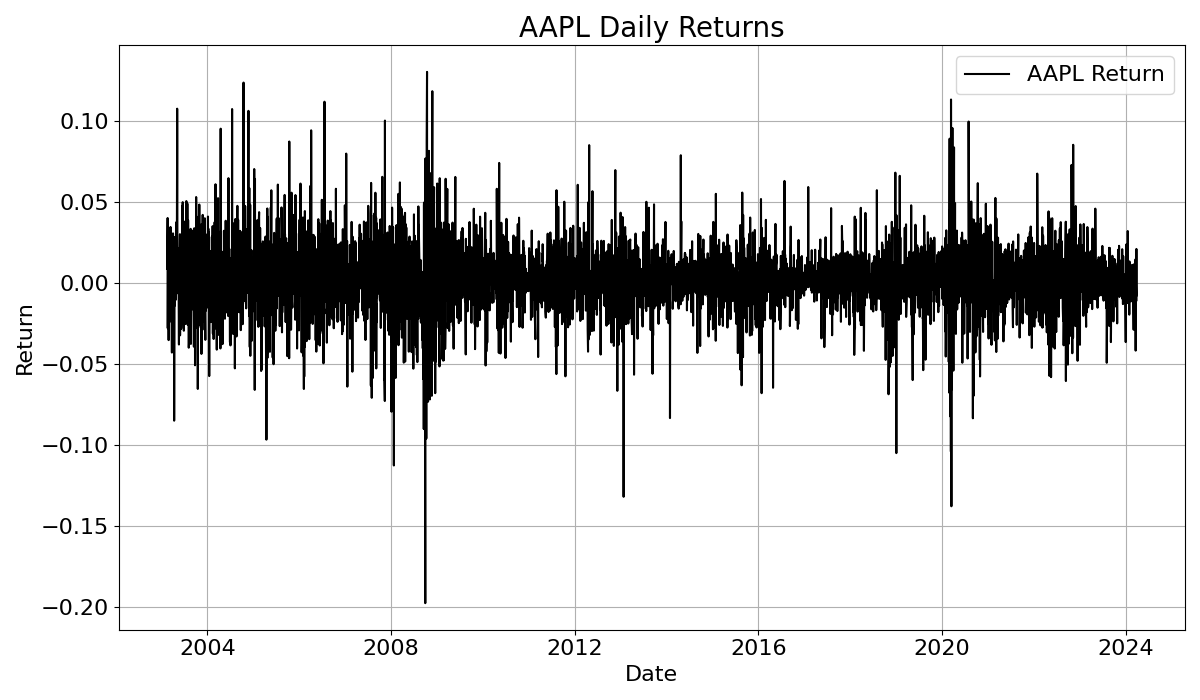
\includegraphics[width=\linewidth, height=5cm]{Images/Data/descriptive_statistics_AAPL_daily_return_plot.png}
        \caption{Time-series of AAPL daily returns from 2003 to 2024}
        \label{fig:descriptive_statistics_AAPL_daily_return_plot}
    \end{subfigure}
    \hfill
    \begin{subfigure}[b]{0.49\textwidth}
        \centering
        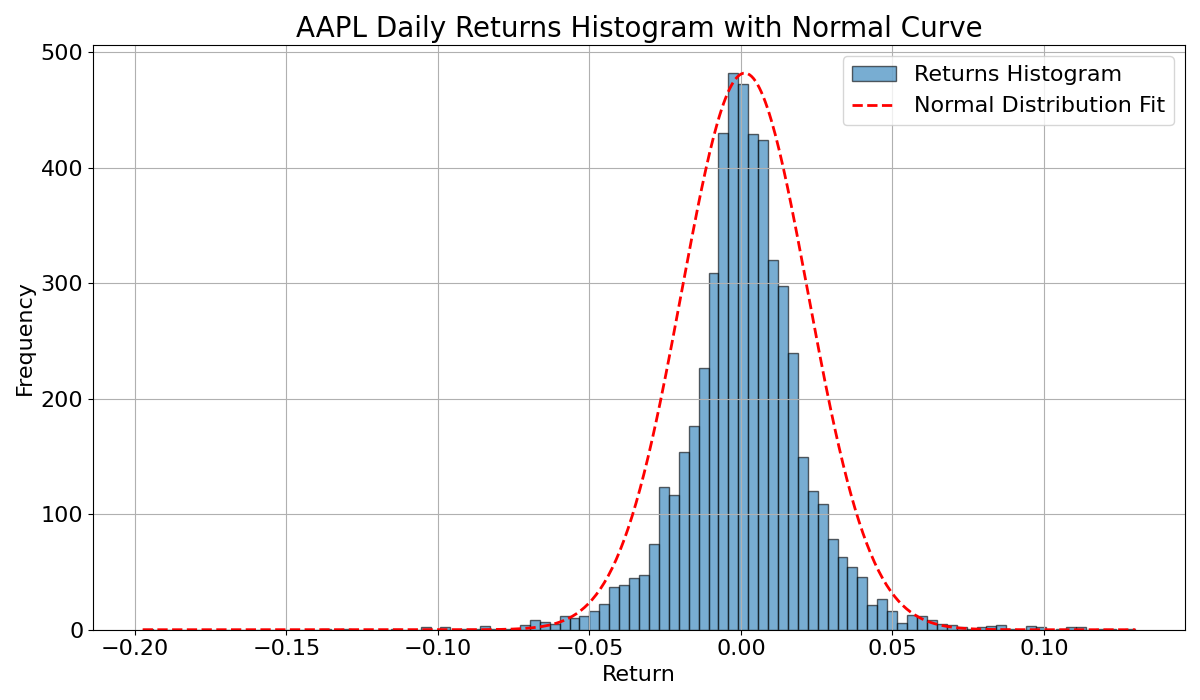
\includegraphics[width=\linewidth, height=5cm]{Images/Data/descriptive_statistics_AAPL_daily_return_histogram.png}
        \caption{Histogram of AAPL daily returns with overlaid normal distribution}
        \label{fig:descriptive_statistics_AAPL_daily_return_histogram}
    \end{subfigure}
    \caption{Descriptive analysis of AAPL daily returns}
    \label{fig:descriptive_analysis_of_AAPL_daily_returns}
\end{figure}

\begin{figure}[H]
    \centering
    \begin{subfigure}[b]{0.49\textwidth}
        \centering
        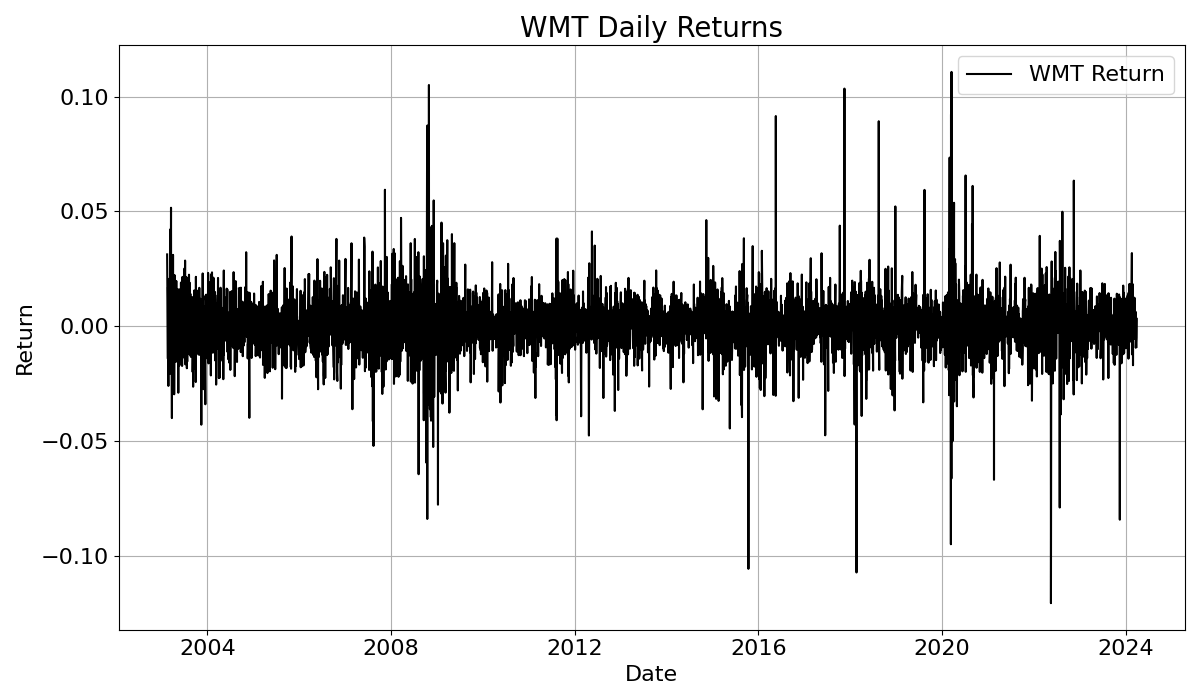
\includegraphics[width=\linewidth, height=5cm]{Images/Data/descriptive_statistics_WMT_daily_return_plot.png}
        \caption{Time-series of WMT daily returns from 2003 to 2024}
        \label{fig:descriptive_statistics_WMT_daily_return_plot}
    \end{subfigure}
    \hfill
    \begin{subfigure}[b]{0.49\textwidth}
        \centering
        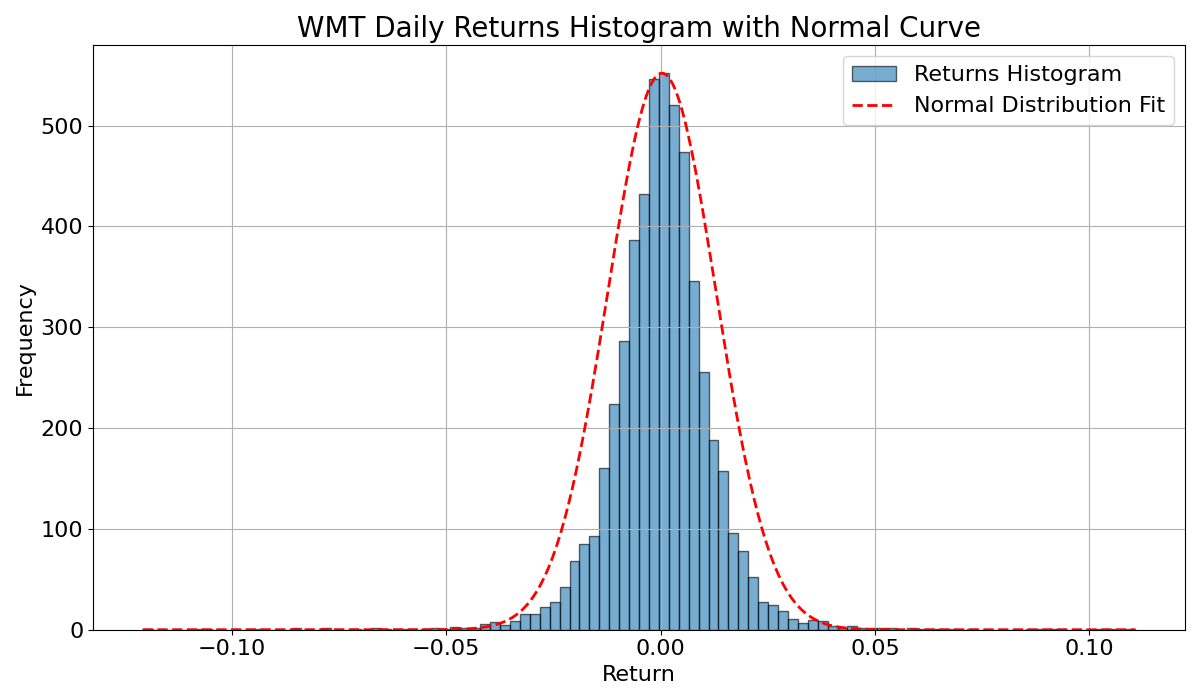
\includegraphics[width=\linewidth, height=5cm]{Images/Data/descriptive_statistics_WMT_daily_return_histogram.png}
        \caption{Histogram of WMT daily returns with overlaid normal distribution.}
        \label{fig:descriptive_statistics_WMT_daily_return_histogram}
    \end{subfigure}
    \caption{Descriptive analysis of WMT daily returns}
    \label{fig:descriptive_analysis_of_WMT_daily_returns}
\end{figure}

\subsection{Diagnostic Tests}
\label{sec:diagnostic_tests}
To better understand the statistical properties of the return series for the individual stocks, several diagnostic tests are conducted. Firstly, the Augmented Dickey-Fuller \parencite{Dickey1981} test shows stationarity across all return series at the 1\% significance level. Secondly, the ARCH-LM test \parencite{Engle1982} detects autoregressive conditional heteroskedasticity in all series at the same significance level, indicating  significant volatility clustering. Further, Jarque-Bera \parencite{Jarque1980} tests reject the null of normality for all raw return series with 1\% significance, suggesting that incorporating benchmark models with heavy-tailed or non-normal distributions is appropriate. Finally, the Ljung-Box \parencite{LJUNG1978} test, conducted with 20 lags reveals significant serial correlation in both raw and squared returns for the majority of stocks. While autocorrelation in squared returns is expected due to volatility clustering, the presence of serial correlation in raw returns for most series indicates linear dependencies. Consequently, GARCH models incorporating ARMA terms in the mean equation are justified and subsequently included in the benchmarking framework.

% ==================== Feature Engineering ==================== %
\subsection{Feature Engineering and Preprocessing}
\label{sec:feature_engineering}
Daily returns are log transformed for each stock such that $r_{t,i} = log(P_t/P_{t-1})$, representing the log return at day $t$ for stock $i$, becomes the dependent variable. The use of log returns is standard in financial econometrics due to their additive properties over time and their ability to stabilize variance and approximate continuously compounded returns (Cont2001).

Further, realized variance (RV), realized quarticity (RQ), and implied volatility (IV) are provided in the datasets in annualized percentage units. To ensure comparability and facilitate meaningful learning by the model, these measures are transformed into daily log variance or quarticity expressed in decimal form. The transformations follow standard variance scaling procedures, which involve adjusting for the number of trading days in a year—252.

The scaled and log-transformed inputs are defined as follows: 


\begin{equation*}
    \begin{gathered}
  \text{RV}_{\text{daily}} \sim  \log\left( \frac{\text{RV}_{\text{annual}}}{100^2 \cdot 252} + \varepsilon \right), \; \;
  \text{RQ}_{\text{daily}} \sim \log\left( \frac{\text{RQ}_{\text{annual}}}{100^2 \cdot 252^2} + \varepsilon \right), \; \;
    \text{IV}_{\text{daily}} \sim \log\left( \frac{\text{IV}_{\text{annual}}^2}{100^2 \cdot 252} + \varepsilon \right) \\
    \end{gathered}
\end{equation*}

Here, $\epsilon = 1e^{-12}$ is a small positive constant added for numerical stability, preventing undefined values in the event of extremely low or zero inputs.

Missing values in the selected features are handled using forward filling within each stocks time series. This method carries forward the last observed value to fill missing entries, preserving the temporal structure and avoiding look-ahead bias, critical for correctness in time series forecasting.

\begin{comment}
   The models utilize transformed variants of the input feature from the dateset. (This is to ensure consistency in scaling.. el.?). All volatility-related variables—realized volatility (RV), bipower variation (BVP), as well as good (Good) and bad (Bad) volatility—in addition to implied volatility (IVOL) variables, are transformed from annualized volatility percentage to daily log-variance. [REASON AND SOURCE FOR WHY]. 
Target variable is log-return...
Realized quatizity (RQ), originally provided as annualized fourth power percentage measure, are transformed to daily level and log-transformed.
No additional features or transformations are applied beyond these volatility measures.  

- Transformation of RV, RQ and IV /252 (training days) / 100 decimal..  
\end{comment}





% ==================== Data Preprocessing ==================== % 
\subsection{Data Split}
\label{sec:data_preprocessing}
To ensure robust model validation, the dataset is partitioned into distinct training, validation, and test sets. The training set contains observations up to \trainSetEnd. The training set includes all observations up to \trainSetEnd, while the validation set spans the period from \trainSetEnd to \validationSetEnd and is used to tune model parameters and monitor performance during development. The test set, covering \validationSetEnd to \testSetEnd, is reserved for final out-of-sample evaluation. 

Maintaining a separate and entirely unseen test set ensures that model selection and tuning are not influenced by test performance, thereby preventing overfitting and preserving the validity of the evaluation. This practice supports the integrity and credibility of the reported performance metrics by ensuring that the test results reflect true generalization ability rather than optimization on the test data \parencite{hyndman2018forecasting}. Moreover, a sufficiently long test period is necessary for the reliability of ES backtesting. Short evaluation windows can produce misleading results due to limited tail events, thus undermining the statistical power of backtesting procedures \parencite{Bayer2020}. A longer test horizon also enables performance evaluation across varying market regimes, including periods of both high and low volatility. This is particularly important in financial applications, where model robustness and adaptability to changing conditions are essential—both from a practical forecasting perspective and for regulatory bodies.

This partitioning framework therefore enhances the empirical credibility of the study and enables sound inference regarding the predictive performance of the probabilistic AI models under consideration.

\begin{comment}
    To ensure robust model validation, the dataset is partitioned into distinct training, validation and test sets. The training set comprises data up to \trainSetEnd. The validation set contains data from \validationSetStart to \validationSetEnd and is used for XXX. The final test set is reserved for out-of-sample evaluation to assess the prediction performance of the probabilistic AI models, and spans from \testSetStart to \datasetDJIEnd. [Source on the split ratio and how much data in each]

... Having a separate test set that remains unseen until final models are selected ensures robustness because the models are not trained to overfit on the test period. This also enhances the validness of the results and therefore ability to draw conclusions or something something ... 
\end{comment}

